%==============================================================================
% Tento soubor použijte jako základ
% This file should be used as a base for the thesis
% Autoři / Authors: 2008 Michal Bidlo, 2022 Jaroslav Dytrych
% Kontakt pro dotazy a připomínky: sablona@fit.vutbr.cz
% Contact for questions and comments: sablona@fit.vutbr.cz
%==============================================================================
% kódování: UTF-8 (zmena prikazem iconv, recode nebo cstocs)
% encoding: UTF-8 (you can change it by command iconv, recode or cstocs)
%------------------------------------------------------------------------------
% zpracování / processing: make, make pdf, make clean
%==============================================================================
% Soubory, které je nutné upravit nebo smazat: / Files which have to be edited or deleted:
%   documentation-20-literatura-bibliography.bib - literatura / bibliography
%   documentation-01-kapitoly-chapters.tex - obsah práce / the thesis content
%   documentation-01-kapitoly-chapters-en.tex - obsah práce v angličtině / the thesis content in English
%   projekt-30-prilohy-appendices.tex - přílohy / appendices
%   projekt-30-prilohy-appendices-en.tex - přílohy v angličtině / appendices in English
%==============================================================================
\documentclass[]{fitthesis} % bez zadání - pro začátek práce, aby nebyl problém s překladem
%\documentclass[english]{fitthesis} % without assignment - for the work start to avoid compilation problem
%\documentclass[zadani]{fitthesis} % odevzdani do IS VUT a/nebo tisk s barevnými odkazy - odkazy jsou barevné
%\documentclass[english,zadani]{fitthesis} % for submission to the IS VUT and/or print with color links - links are color
%\documentclass[zadani,print]{fitthesis} % pro černobílý tisk - odkazy jsou černé
%\documentclass[english,zadani,print]{fitthesis} % for the black and white print - links are black
%\documentclass[zadani,cprint]{fitthesis} % pro barevný tisk - odkazy jsou černé, znak VUT barevný
%\documentclass[english,zadani,cprint]{fitthesis} % for the print - links are black, logo is color
% * Je-li práce psaná v anglickém jazyce, je zapotřebí u třídy použít 
%   parametr english následovně:
%   If thesis is written in English, it is necessary to use 
%   parameter english as follows:
%      \documentclass[english]{fitthesis}
% * Je-li práce psaná ve slovenském jazyce, je zapotřebí u třídy použít 
%   parametr slovak následovně:
%   If the work is written in the Slovak language, it is necessary 
%   to use parameter slovak as follows:
%      \documentclass[slovak]{fitthesis}
% * Je-li práce psaná v anglickém jazyce se slovenským abstraktem apod., 
%   je zapotřebí u třídy použít parametry english a enslovak následovně:
%   If the work is written in English with the Slovak abstract, etc., 
%   it is necessary to use parameters english and enslovak as follows:
%      \documentclass[english,enslovak]{fitthesis}

% Základní balíčky jsou dole v souboru šablony fitthesis.cls
% Basic packages are at the bottom of template file fitthesis.cls
% zde můžeme vložit vlastní balíčky / you can place own packages here


% Pro seznam zkratek lze využít balíček Glossaries - nutno odkomentovat i níže a při kompilaci z konzoly i v Makefile (plnou verzi pro Perl, nebo lite)
% The Glossaries package can be used for the list of abbreviations - it is necessary to uncomment also below. When compiling from the console also in the Makefile (full version for Perl or lite)
%\usepackage{glossaries}
%\usepackage{glossary-superragged}
%\makeglossaries 

% Nastavení cesty k obrázkům
% Setting of a path to the pictures
%\graphicspath{{obrazky-figures/}{./obrazky-figures/}}
%\graphicspath{{obrazky-figures/}{../obrazky-figures/}}

%---rm---------------
\renewcommand{\rmdefault}{lmr}%zavede Latin Modern Roman jako rm / set Latin Modern Roman as rm
%---sf---------------
\renewcommand{\sfdefault}{qhv}%zavede TeX Gyre Heros jako sf
%---tt------------
\renewcommand{\ttdefault}{lmtt}% zavede Latin Modern tt jako tt

% vypne funkci šablony, která automaticky nahrazuje uvozovky,
% aby nebyly prováděny nevhodné náhrady v popisech API apod.
% disables function of the template which replaces quotation marks
% to avoid unnecessary replacements in the API descriptions etc.
\csdoublequotesoff

\usepackage{url}

% =======================================================================
% balíček "hyperref" vytváří klikací odkazy v pdf, pokud tedy použijeme pdflatex
% problém je, že balíček hyperref musí být uveden jako poslední, takže nemůže
% být v šabloně
% "hyperref" package create clickable links in pdf if you are using pdflatex.
% Problem is that this package have to be introduced as the last one so it 
% can not be placed in the template file.
\ifWis
\ifx\pdfoutput\undefined % nejedeme pod pdflatexem / we are not using pdflatex
\else
  \usepackage{color}
  \usepackage[unicode,colorlinks,hyperindex,plainpages=false,pdftex]{hyperref}
  \definecolor{hrcolor-ref}{RGB}{223,52,30}
  \definecolor{hrcolor-cite}{HTML}{2F8F00}
  \definecolor{hrcolor-urls}{HTML}{092EAB}
  \hypersetup{
	linkcolor=hrcolor-ref,
	citecolor=hrcolor-cite,
	filecolor=magenta,
	urlcolor=hrcolor-urls
  }
  \def\pdfBorderAttrs{/Border [0 0 0] }  % bez okrajů kolem odkazů / without margins around links
  \pdfcompresslevel=9
\fi
\else % pro tisk budou odkazy, na které se dá klikat, černé / for the print clickable links will be black
\ifx\pdfoutput\undefined % nejedeme pod pdflatexem / we are not using pdflatex
\else
  \usepackage{color}
  \usepackage[unicode,colorlinks,hyperindex,plainpages=false,pdftex,urlcolor=black,linkcolor=black,citecolor=black]{hyperref}
  \definecolor{links}{rgb}{0,0,0}
  \definecolor{anchors}{rgb}{0,0,0}
  \def\AnchorColor{anchors}
  \def\LinkColor{links}
  \def\pdfBorderAttrs{/Border [0 0 0] } % bez okrajů kolem odkazů / without margins around links
  \pdfcompresslevel=9
\fi
\fi
% Řešení problému, kdy klikací odkazy na obrázky vedou za obrázek
% This solves the problems with links which leads after the picture
\usepackage[all]{hypcap}


% Informace o práci/projektu / Information about the thesis
%---------------------------------------------------------------------------
\projectinfo{
  %Prace / Thesis
  project={SP},            %typ práce BP/SP/DP/DR  / thesis type (SP = term project)
  year={2024},             % rok odevzdání / year of submission
  date=\today,             % datum odevzdání / submission date
  %Nazev prace / thesis title
  title.cs={Demonstrace ovládání TFT displeje přes\\Wi\nobreak Fi/Bluetooth},  % název práce v češtině či slovenštině (dle zadání) / thesis title in czech language (according to assignment)
  title.en={Demonstration of TFT display control via WiFi/Bluetooth}, % název práce v angličtině / thesis title in english
  %title.length={14.5cm}, % nastavení délky bloku s titulkem pro úpravu zalomení řádku (lze definovat zde nebo níže) / setting the length of a block with a thesis title for adjusting a line break (can be defined here or below)
  %sectitle.length={14.5cm}, % nastavení délky bloku s druhým titulkem pro úpravu zalomení řádku (lze definovat zde nebo níže) / setting the length of a block with a second thesis title for adjusting a line break (can be defined here or below)
  %dectitle.length={14.5cm}, % nastavení délky bloku s titulkem nad prohlášením pro úpravu zalomení řádku (lze definovat zde nebo níže) / setting the length of a block with a thesis title above declaration for adjusting a line break (can be defined here or below)
  %Autor / Author
  author.name={Michal},   % jméno autora / author name
  author.surname={Blažek},   % příjmení autora / author surname 
  %author.title.p={Bc.}, % titul před jménem (nepovinné) / title before the name (optional)
  %author.title.a={Ph.D.}, % titul za jménem (nepovinné) / title after the name (optional)
  %Ustav / Department
  department={UPSY}, % doplňte příslušnou zkratku dle ústavu na zadání: UPSY/UIFS/UITS/UPGM / fill in appropriate abbreviation of the department according to assignment: UPSY/UIFS/UITS/UPGM
  % Školitel / supervisor
  supervisor.name={Václav},   % jméno školitele / supervisor name 
  supervisor.surname={Šimek},   % příjmení školitele / supervisor surname
  supervisor.title.p={Ing.},   %titul před jménem (nepovinné) / title before the name (optional)
  % supervisor.title.a={Ph.D.},    %titul za jménem (nepovinné) / title after the name (optional)
}

% nastavení délky bloku s titulkem pro úpravu zalomení řádku - lze definovat zde nebo výše / setting the length of a block with a thesis title for adjusting a line break - can be defined here or above
%\titlelength{14.5cm}
% nastavení délky bloku s druhým titulkem pro úpravu zalomení řádku - lze definovat zde nebo výše / setting the length of a block with a second thesis title for adjusting a line break - can be defined here or above
%\sectitlelength{14.5cm}
% nastavení délky bloku s titulkem nad prohlášením pro úpravu zalomení řádku - lze definovat zde nebo výše / setting the length of a block with a thesis title above declaration for adjusting a line break - can be defined here or above
%\dectitlelength{14.5cm}

% řeší první/poslední řádek odstavce na předchozí/následující stránce
% solves first/last row of the paragraph on the previous/next page
\clubpenalty=10000
\widowpenalty=10000

% checklist
\newlist{checklist}{itemize}{1}
\setlist[checklist]{label=$\square$}

% Kompilace po částech (rychlejší, ale v náhledu nemusí být vše aktuální)
% Compilation piecewise (faster, but not all parts in preview will be up-to-date)
% Další informace viz / For more information see https://www.overleaf.com/learn/latex/Multi-file_LaTeX_projects
% \usepackage{subfiles}

% Nechcete-li, aby se u oboustranného tisku roztahovaly mezery pro zaplnění stránky, odkomentujte následující řádek / If you do not want enlarged spacing for filling of the pages in case of duplex printing, uncomment the following line
% \raggedbottom

\usepackage{fvextra}

\begin{document}
  % Vysazeni titulnich stran / Typesetting of the title pages
  % ----------------------------------------------
  \maketitle
  % Obsah
  % ----------------------------------------------
  \setlength{\parskip}{0pt}

  {\hypersetup{hidelinks}\tableofcontents}
  
  % Seznam obrazku a tabulek (pokud prace obsahuje velke mnozstvi obrazku, tak se to hodi)
  % List of figures and list of tables (if the thesis contains a lot of pictures, it is good)
  
  % {\hypersetup{hidelinks}\listoftables}

  % Seznam zkratek / List of abbreviations
  %\ifczech
  %  \renewcommand*\glossaryname{Seznam zkratek}%
  %  \renewcommand*\entryname{Zkratka}
  %  \renewcommand*\descriptionname{Význam}
  %\fi
  %\ifslovak
  %  \renewcommand*\glossaryname{Zoznam skratiek}%
  %  \renewcommand*\entryname{Skratka}
  %  \renewcommand*\descriptionname{Význam}
  %\fi
  %\ifenglish
  %  \renewcommand*\glossaryname{List of abbreviations}%
  %  \renewcommand*\entryname{Abbreviation}
  %  \renewcommand*\descriptionname{Meaning}
  %\fi
  % Definice zkratek - z textu se odkazují např. \Gls{TF–IDF}
  % Definition of abbreviations - referred from the text e.g. \Gls{TF–IDF}
  %\newglossaryentry{TF–IDF}
  %{
  %  name={TF–IDF},
  %  description={Term Frequency-Inverse Document Frequency}
  %}
  % 
  %\setglossarystyle{superragged}
  %\printglossaries


  \ifODSAZ
    \setlength{\parskip}{0.5\bigskipamount}
  \else
    \setlength{\parskip}{0pt}
  \fi

  % vynechani stranky v oboustrannem rezimu
  % Skip the page in the two-sided mode
  \iftwoside
    \cleardoublepage
  \fi

  % Text prace / Thesis text
  % ----------------------------------------------
  \ifenglish
    \input{documentation-01-kapitoly-chapters-en}
  \else
    \chapter{Úvod}

Tato práce se zaměřuje na ovládání barevného TFT displeje, připojeného k~vývojovému kitu ESP32, přes rozhraní WiFi nebo Bluetooth. Jelikož zadání povoluje výběr mezi komunikací přes WiFi a Bluetooth, pro tento projekt byla zvolena komunikace přes Bluetooth z~důvodu jednoduchého párování a přímočaré komunikaci mezi dvěma zařízeními. Avšak v~kapitole \ref{sec:test} je zmíněna i negativní stránka připojení přes Bluetooth, a to je nízký objem dat na paket, který zařízení přijímá. Ovládání je demonstrováno na možnosti vypsání textu na displej, vykreslení přijatého obrázku, nebo na možnosti hraní Tetrisu.

Veškerou funkcionalitu demonstruje následující video: \url{https://youtu.be/RHHq2XagPnQ}

\chapter{Návrh}

V~této kapitole je popsán návrh celého projektu od hardwarové části až po samotný kód. Cílem návrhu bylo vytvořit projekt, který umožní ovládání TFT displeje skrze rozhraní WiFi nebo Bluetooth, přičemž v~tomto projektu byla zvolena komunikace přes Bluetooth z~důvodu její přímočaré komunikace mezi dvěma zařízeními. Návrh v~sobě zahrnuje způsob ovládání výsledného projektu a toho je docíleno pomocí externí aplikace \cite{AppPixelBluetoothCanvas}.

\section{Hardware}

V~projektu je použit vývojový kit ESP32 Wemos D1 R32, který přes SPI rozhraní komunikuje s~1,44''~$128\times128$ TFT displejem s~označením ILI9163C.
Pro komunikaci s~počítačem nebo jiným zařízení s~podporou Bluetooth projekt využívá Bluetooth čip, který je součástí vývojového kitu, a tudíž nemusí být externě dodán.

\section{Schéma zapojení}

Na obrázku \ref{fig:zapojeni} je vyfocené zapojení TFT displeje k~vývojovému kitu ESP32. Podrobněji je zapojení jednotlivých pinů v~tabulce \ref{tab:esp32_tft_piny}. Jedná se o~komunikaci přes SPI rozhraní kde ESP32 je \textit{master} a TFT displej je \textit{slave}.

\begin{table}[h!]
    \centering
    \begin{tabular}{|c|c|c|}
        \hline
        \textbf{ESP32 pin}  & \textbf{TFT pin} & \textbf{Popis} \\
        \hline
        3.3V                & VCC              & Napájení 3.3V \\
        \hline
        3.3V                & LED              & Podsvícení displeje \\
        \hline
        GND                 & GND              & Zem \\
        \hline
        IO23                & SDA              & Master Out Slave In (SPI data) \\
        \hline
        IO18                & SCK              & SPI hodiny \\
        \hline
        IO5                 & CS               & Chip Select  \\
        \hline
        IO2                 & DC               & Data/Command \\
        \hline
        IO27                & RST              & Reset displeje \\
        \hline
    \end{tabular}
    \caption{Zapojení jednotlivých pinů vývojového kitu ESP32 na piny TFT displeje.}
    \label{tab:esp32_tft_piny}
\end{table}

\begin{figure}[h!]
    \centering
    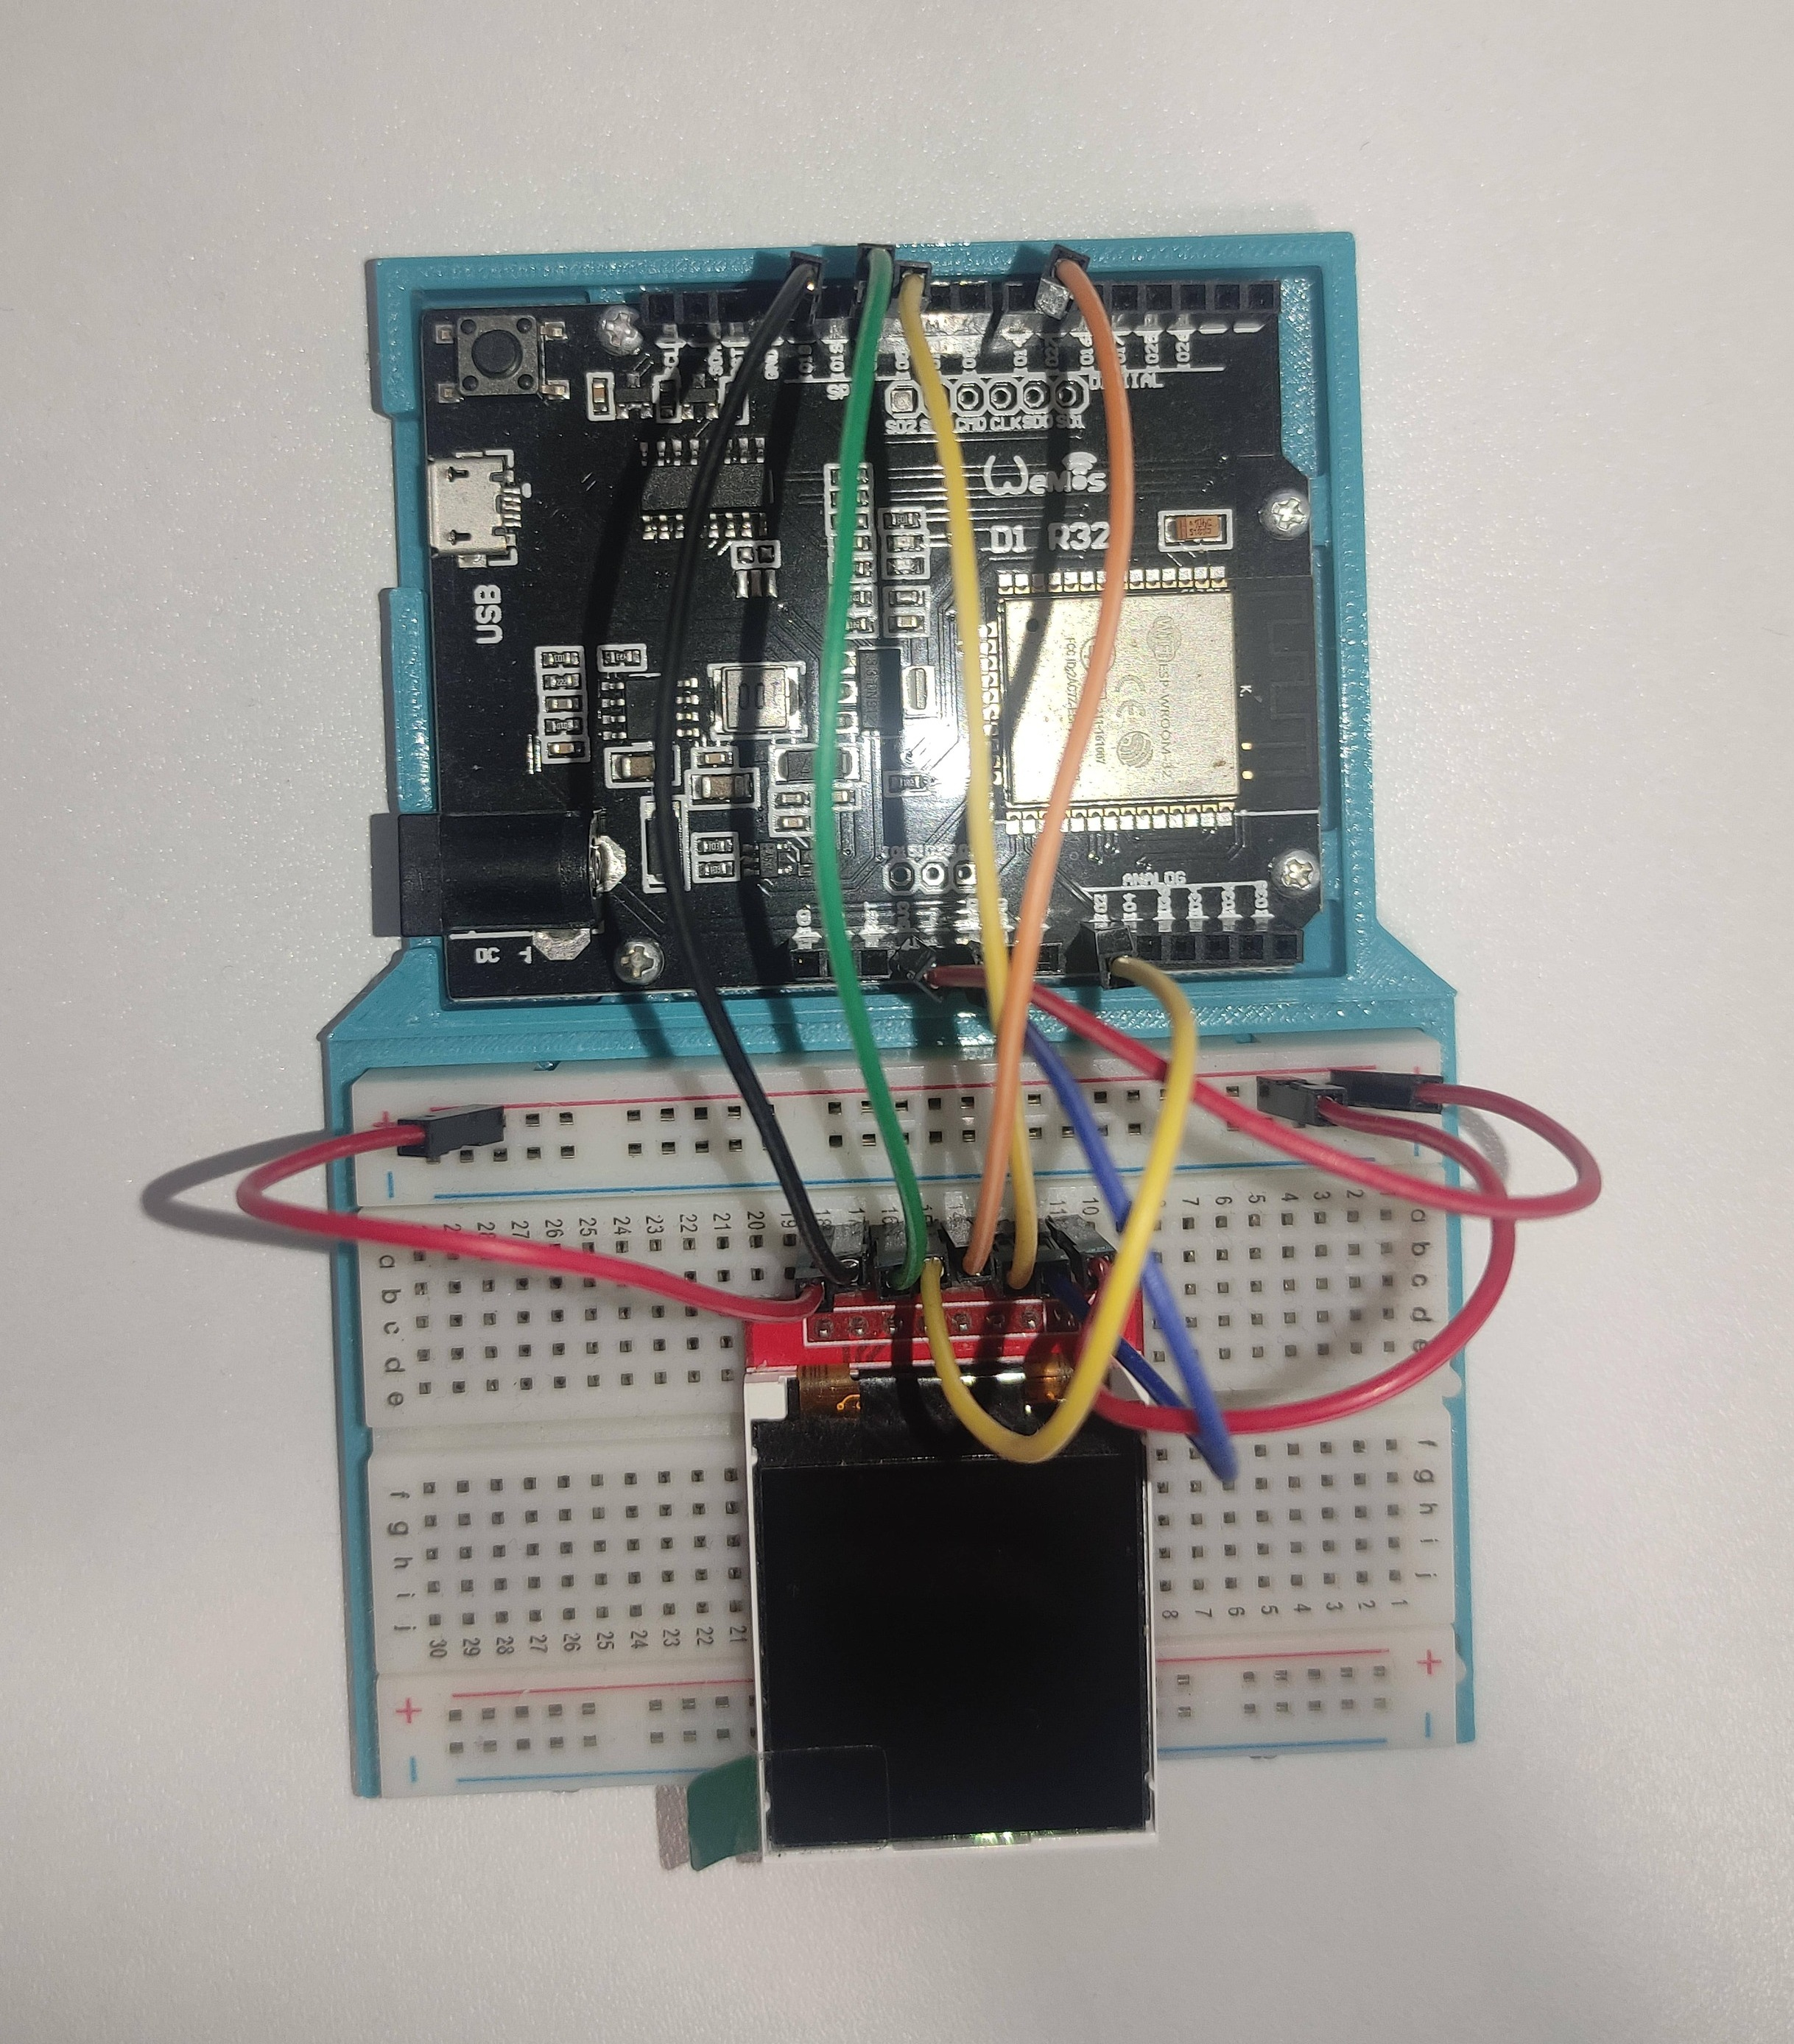
\includegraphics[width=0.7\linewidth]{obrazky-figures/wiring.jpg}
    \caption{Zobrazení zapojení TFT displeje k~vývojovému kitu ESP32.}
    \label{fig:zapojeni}
\end{figure}

\section{Vývojové prostředí}

Vývoj programu se uskutečnil v~aplikaci \texttt{vscode} s~rozšířením \texttt{PlatformIO}, které bez problému automaticky nalezlo připojený vývojový kit a nahrálo do něj nový program. Veškerý vývoj probíhal v~Linuxovém prostředí na operačním systému Ubuntu 24.04.1 LTS.

V~tomto projektu je použit Arduino framework z~důvodu kompatibility s~externími knihovnami a z~důvodu použití programovacího jazyka C++, ve kterém je následně implementovaný program. Konkrétní části programu využívají prostředků jazyka C++ jako jsou například třídy.

\chapter{Vlastnosti programu}

Program je rozdělen na 3 hlavní funkcionality. V~první pouze vykreslí text, který obdržel přes Bluetooth, na TFT displej. Toho je docíleno za pomoci metody \texttt{print} z~externí knihovny \textit{Adafruit GFX}.

Druhá funkcionalita je vykreslení obrázku. Tento obrázek se posílá po několika částech z~důvodu přetečení zásobníku pro přijatá data skrz Bluetooth komunikaci. Pokud by zásobník přetekl, některá data by se ztratila a obrázek by vypadal jinak, než by bylo očekáváno. Vykreslení obrázků je nejjemnější možné, takže lze změnit barvu každého pixelu displeje, a to až na 65 tisíc různých barev, protože se využívá dvou bajtů barvy ve formátu RGB565.

Poslední hlavní funkcionalita je hra Tetris, která se spouští, jakmile vývojový kit detekuje zmáčknutí tlačítka doleva nebo doprava. Následně lze pohybovat s~padajícími tvary pomocí těchto šipek. Pokud uživatel prohraje, obarví se mu rámeček okolo celého displeje červeně a hra se pozastaví. Z~tohoto pozastaveného bodu a vlastně kdykoliv během hry se dá odejít pomocí přijetí dalších dat, které mají buďto zobrazit obrázek, nebo vykreslit text.

Obě strany komunikace musí mít stejně definovaný tvar bajtů, které mezi sebou přenáší. V~tomto případě je tato informace v~tabulce \ref{tab:bajty}. Vývojový kit se na základě prvního bajtu celé zprávy rozhodne, zda má vypsat text, vykreslit obrázek nebo spustit hru Tetris.

\begin{table}[h!]
    \centering
    \begin{tabular}{|l|p{46mm}|p{50mm}|}
        \hline
        \textbf{Příkaz v~aplikaci}  & \textbf{Formát odesílaných dat}       & \textbf{Popisek} \\
        \hline
        Obrázek (1. část)           & 0x00 \uv{data obrázku}                & 0x00 bajt na začátku dat určuje informaci, že se bude nahrávat nový obrázek. \\
        \hline
        Obrázek (ostatní části)     & 0x01 \uv{data obrázku}                & 0x01 bajt na začátku dat určuje informaci, že obrázek má i další část. \\
        \hline
        Text                        & 0x02 \uv{text ze vstupuního pole}     & 0x02 bajt na začátku dat určuje informaci, že tato data jsou text. \\
        \hline
        Tlačítko s~levou šipkou     & 0x03                                  & Přijme pouze jeden bajt, a to 0x03. \\
        \hline
        Tlačítko s~pravou šipkou    & 0x04                                  & Přijme pouze jeden bajt, a to 0x04. \\
        \hline
    \end{tabular}
    \caption{Jednotlivé zprávy v~bajtech pro komunikaci mezi vývojovým kitem a testovací aplikací \cite{AppPixelBluetoothCanvas}.}
    \label{tab:bajty}
\end{table}

\section{Testování}
\label{sec:test}

Testování probíhalo skrze aplikaci \cite{AppPixelBluetoothCanvas}, která posílá data ve správném formátu přes Bluetooth na výukový kit ESP32. Tato aplikace se pomocí Bluetooth adresy vývojového kitu s~ním spáruje a poté na něj odesílá data. Nejdříve zpracovává nakreslený obraz, napsaný text nebo zmáčknuté tlačítko do bajtových instrukcí, které se poté pošlou na ESP32 a vývojový kit následně podle prvního bajtu určí následující sekvenci instrukcí, která se provede.

Z~testů bylo zjištěno, že Bluetooth má zásobník ne přijatá data a pokud dostane příliš moc dat, nebo je dostává rychleji než zpracovává, může dojít k~přetečení a ke ztrátě dat. Toto se výrazně projevuje u~obrázku, tudíž jsou tyto obrázky posílány po částech, kde program nejdříve zpracuje první část a až po nějaké chvilce mu přijdou data na druhou část. Z~většiny toto vyřešilo zmíněný problém, avšak někdy se data stejně ztratí. V~tomto případě je doporučeno proces opakovat a nahrát obrázek znovu.

\chapter{Závěr}

Program ve spojení s~aplikací \cite{AppPixelBluetoothCanvas} funguje skvěle a zvládne zobrazit text, či nakreslený obrázek. Všechna data se mezi počítačem a vývojovým kitem ESP32 odesílají pomocí Bluetooth a poté skrze SPI rozhraní zobrazují na TFT displeji.

Program by se určitě dal vylepšit minimálně ze strany Tetrisu o~chybějící rotace tvarů. Ačkoliv je implementováno odebírání zaplněné řady a posunutí všech čtverečků nad touto řadou, nelze to jednoduše dokázat a obecně hraní Tetrisu bez možnosti otočit právě padající dílek není úplně příjemné.

\section*{Výsledek autoevaluace}

Zadání vyžaduje autoevaluaci vlastního projektu a to je zobrazeno níže v~tabulce \ref{tab:autoevaluace}.

\begin{table}[h!]
    \centering
    \begin{tabular}{|l|p{62mm}|c|}
        \hline
        \textbf{Položka} & \textbf{Popis hodnocení} & \textbf{Očekávané body} \\
        \hline
        E (Přístup k~řešení)     & Dostatečný zájem k~řešení projektu s~implementováním Tetrisu nad rámec zadání. & 2/2 \\
        \hline
        F (Funkčnost řešení)     & Funkčnost zadání splněna. & 5/5 \\
        \hline
        Q (Kvalita řešení)       & Splňuje všechno potřebné ze zadání s~menším nedostatkem, a to použitím Arduino frameworku. & 1/2 \\
        \hline
        P (Prezentace)           & Video ukazuje všechno potřebné včetně složitějšího zaplnění řady v~Tetrise a jejího následného smazání se zhoršenou kvalitou. & 1,5/2 \\
        \hline
        D (Dokumentace k~řešení) & Dokumentace má samozřejmě svoje chyby, ale základní struktura je dostatečně splněna. & 2,5/3 \\
        \hline
    \end{tabular}
    \caption{Autoevaluace projektu podle hodnoticího klíče z~\cite{HodnoticiKlic}.}
    \label{tab:autoevaluace}
\end{table}

  \fi
  
  % Kompilace po částech (viz výše, nutno odkomentovat a zakomentovat input výše)
  % Compilation piecewise (see above, it is necessary to uncomment it and comment out input above)
  %\subfile{chapters/projekt-01-uvod-introduction}
  % ...
  %\subfile{chapters/projekt-05-zaver-conclusion}

  % Pouzita literatura / Bibliography
  % ----------------------------------------------
\ifslovak
  \makeatletter
  \def\@openbib@code{\addcontentsline{toc}{chapter}{Literatúra}}
  \makeatother
  \bibliographystyle{bib-styles/Pysny/skplain}
\else
  \ifczech
    \makeatletter
    \def\@openbib@code{\addcontentsline{toc}{chapter}{Literatura}}
    \makeatother
    \bibliographystyle{bib-styles/Pysny/czplain}
  \else 
    \makeatletter
    \def\@openbib@code{\addcontentsline{toc}{chapter}{Bibliography}}
    \makeatother
    \bibliographystyle{bib-styles/Pysny/enplain}
  %  \bibliographystyle{alpha}
  \fi
\fi
  \begin{flushleft}
  \bibliography{documentation-20-literatura-bibliography}
  \end{flushleft}

  % vynechani stranky v oboustrannem rezimu
  % Skip the page in the two-sided mode
  \iftwoside
    \cleardoublepage
  \fi

  % Prilohy / Appendices
  % ---------------------------------------------
  \appendix
\ifczech
  \renewcommand{\appendixpagename}{Přílohy}
  \renewcommand{\appendixtocname}{Přílohy}
  \renewcommand{\appendixname}{Příloha}
\fi
\ifslovak
  \renewcommand{\appendixpagename}{Prílohy}
  \renewcommand{\appendixtocname}{Prílohy}
  \renewcommand{\appendixname}{Príloha}
\fi
%  \appendixpage

% vynechani stranky v oboustrannem rezimu
% Skip the page in the two-sided mode
%\iftwoside
%  \cleardoublepage
%\fi
  
\ifslovak
%  \section*{Zoznam príloh}
%  \addcontentsline{toc}{section}{Zoznam príloh}
\else
  \ifczech
%    \section*{Seznam příloh}
%    \addcontentsline{toc}{section}{Seznam příloh}
  \else
%    \section*{List of Appendices}
%    \addcontentsline{toc}{section}{List of Appendices}
  \fi
\fi
  \startcontents[chapters]
  \setlength{\parskip}{0pt} 
  % seznam příloh / list of appendices
  % \printcontents[chapters]{l}{0}{\setcounter{tocdepth}{2}}
  
  \ifODSAZ
    \setlength{\parskip}{0.5\bigskipamount}
  \else
    \setlength{\parskip}{0pt}
  \fi
  
  % vynechani stranky v oboustrannem rezimu
  \iftwoside
    \cleardoublepage
  \fi
  
  % Kompilace po částech (viz výše, nutno odkomentovat)
  % Compilation piecewise (see above, it is necessary to uncomment it)
  %\subfile{projekt-30-prilohy-appendices}
  
\end{document}
